\section{実装}
\subsection{maplerubyの基本動作}
入力された値の次の素数を出力するnextprimeを用いて説明する.

\begin{figure}[htbp]\begin{center}
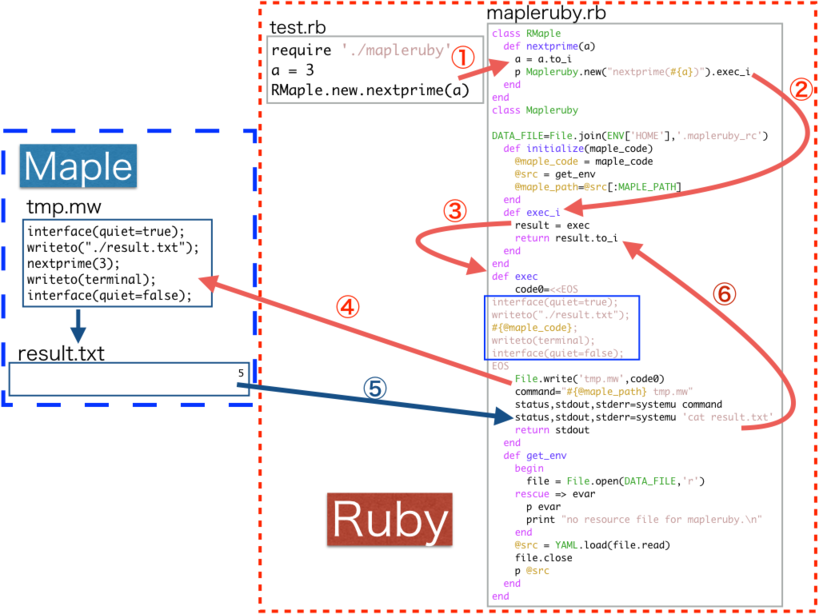
\includegraphics[width=12cm,bb= 0 0 937 753]{../figs/./mapleruby_eringi.003.png}
\caption{maplerubyの基本動作.}
\label{figure:one}
\label{default}\end{center}\end{figure}
\begin{enumerate}
\item maplerubyをrequireした上で使いたい関数を使う.RMaple.new.hogehogeのhogehogeに使いたい関数名を入れる.今回はnextprimeで説明を進める.
\item RMapleクラス内のnextprime関数が呼び出され,aに3が入る.この時nextprimeは入力された値がint型になるように関数内でto\_iしてある.その後,Maplerubyクラスのexec\_i関数へ"nextprime(3)"が出力される.この出力された文字列がそのままMapleでの計算に使われる.
\item 出力された文字列をさらにexec関数へ出力する.
\item 青四角内の内容をMapleへと出力する.この時\verb|#{@maple_code};|となっている部分に先ほどの"nextprime(3)"が入る.青四角の内容がMapleに出力され実行されることで得られた答えがresult.txtに出力されるようになっている.
\item result.txtに出力された内容をRuby側で受け取り,exec\_iに再び返す.
\item 返された値をto\_iすることでint型に直して解を出力する.
\end{enumerate}
\subsection{出力の切り替えの実装例}
先ほどと同様にnextprimeを例に挙げるとexec\_iは,execでmapleに式を送った後mapleから受け取った値をto\_iし,int型にしてから返すようになっている.もし使われた関数が素数判定をtrue/falseで出力するisprimeだった場合は,出力はboolean型が好ましいため受け取った値をboolean型にするexec\_bを用いている.このように整数論に関する関数は,出力に応じてint型で解を得たい場合はexec\_i,float型ならexec\_f,string型ならexec\_sとすることで切り替えられるようになっている.

一方で,行列の場合は出力に切り替えについて例外が存在する.なぜなら,MapleのCUI版は行列の表現が独自のもので,それがresult.txtを通してRubyに出力されるからだ.
例えば,行列を生成する関数matrixは以下のように解を出力する.
\begin{lstlisting}[style=,basicstyle={\scriptsize\ttfamily}]
> with(LinearAlgebra):
> matrix(3,3,[[1,4,7],[2,11,8],[3,6,0]]);
                                             [1     4    7]
                                             [            ]
                                             [2    11    8]
                                             [            ]
                                             [3     6    0]
\end{lstlisting}
この空白部分には半角スペースや改行が入っている上,余分な括弧が付いている.この関数を使う際に行列を生成して出力するだけなら問題ないが計算に数値を使う場合Rubyの方で都合の良い出力型に変える必要がある.そのためのwrapperを考える必要がある.そこで,int型の要素を持つlistlist構造で出力されるのが最も良いと考えた.今回実装した行列の関数の多くは,listlist構造のものをMapleのconvertというlistlist構造からMaple内で扱う行列の形に変換できる関数も一緒にRubyからMapleに送るようにしているためである.行列生成した後理想の型で値を得るためには,いらない記号や空白を取り除き要素をint型にする必要があった.図\ref{figure:two}はmatrixを実装した後,exec\_m(b)というwrapperを作ってみた際に生まれた失敗である.
\newpage

\begin{figure}[htbp]\begin{center}
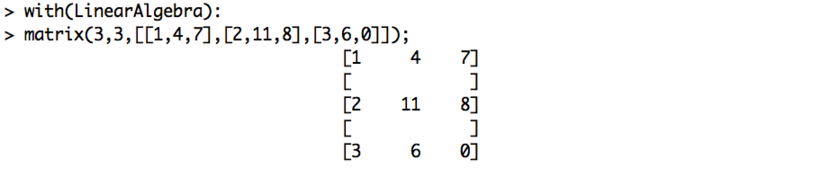
\includegraphics[width=12cm,bb= 0 0 937 753]{../figs/./mapleruby_eringi.004.png}
\caption{exec\_m(b)を実装した際の失敗例.}
\label{figure:two}
\label{default}\end{center}\end{figure}
bには生成した行列の列の数が入る.実装する際に初めに考えたのが図\ref{figure:two}の左側のプログラムである.まずRubyのsplitメソッドを使って1文字ずつに分け,分けた要素全てをint型に変換する.空白はint型に変えた際0になるため,0になった空白部分をdelete\_ifメソッドを用いて削除し,最後にeach\_sliceメソッドを用いて1行目,2行目...と分けてそれぞれ配列に入れ,出力したかった行列と同じようなlistlist構造になるはずだった.しかし,listlist構造への変換はできていたが途中delete\_ifメソッドにより0を消してしまったため,行列の要素で0が含まれていた場合に行列の要素まで消えてしまった.しかも,1文字ずつ分けているため2桁以上の桁数を持つ要素はばらばらになってしまった.

そのことを踏まえて, 図\ref{figure:two}の右側のプログラムを作成した.今度は1文字ずつ分けるところまでは先ほどと一緒で,空白を丸ごと消そうとするのではなくdelete\_ifメソッドで" "(空白),\verb|"\n"|,"[","]"を順番に削除した後にto\_iし,先ほどと同じようにeach\_sliceメソッドでlistlist構造になるようにした.こうしたことによって,要素に0が含まれていてもきちんと出力されるようにはなったが,桁数の問題が残っている.そして,以下の図\ref{figure:three}のように実装することで期待通りに出力を得られるようになった.

\begin{figure}[htbp]\begin{center}
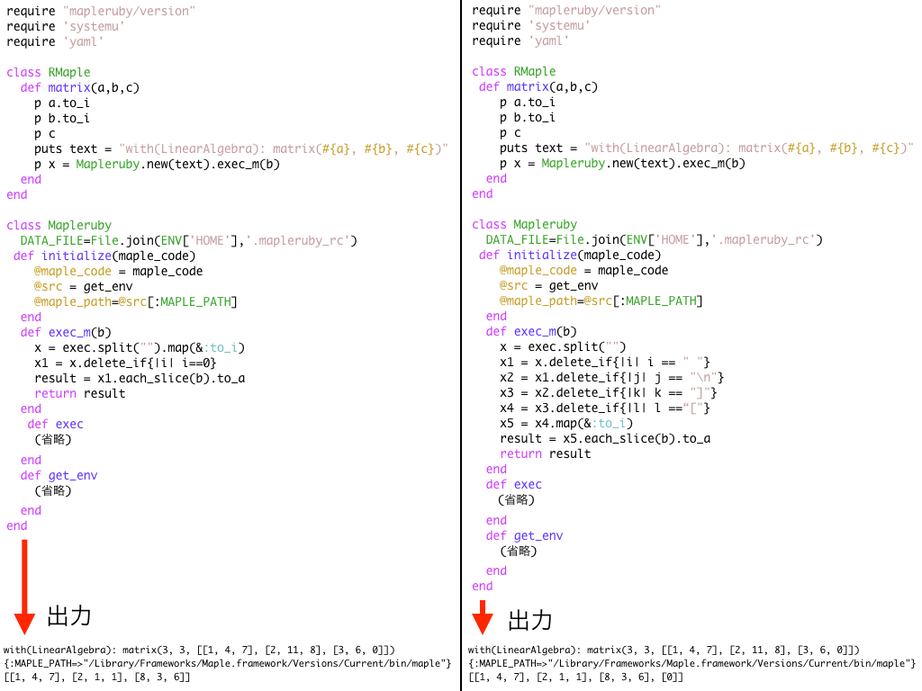
\includegraphics[width=12cm,bb= 0 0 937 753]{../figs/./mapleruby_eringi.005.png}
\caption{exec\_m(b)の完成形.}
\label{figure:three}
\label{default}\end{center}\end{figure}
完成形では,まずgsubメソッドで数字以外の記号を空白に置き換え,splitメソッドで空白を指定することで空白を区切りとした配列にした後int型に直す.直した配列はその後,先ほどと同様にeach\_sliceメソッドを用いてlistlist構造になるようにしている.
\newpage

\subsection{動的メソッドを用いての実装}
一通り実装した後,次に動的メソッドを用いて実装することにより重複コードを減らすように試みたバージョン2を作成した.

\begin{figure}[htbp]\begin{center}
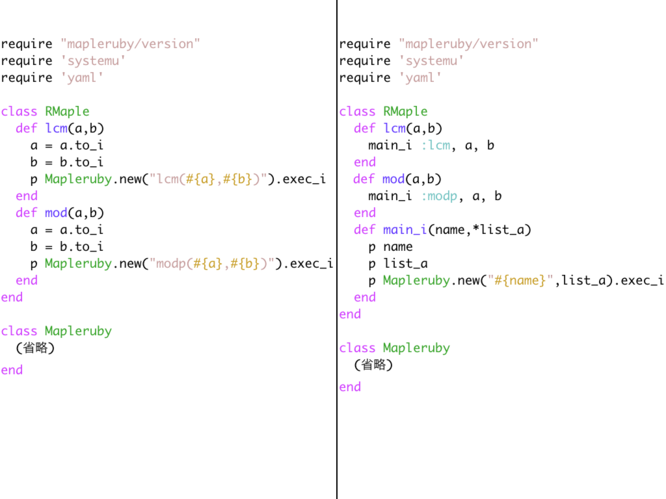
\includegraphics[width=12cm,bb= 0 0 937 753]{../figs/./mapleruby_eringi.006.png}
\caption{左が初期バージョン,右がバージョン2.}
\label{figure:four}
\label{default}\end{center}\end{figure}
初期バージョンでは,関数ごとに各引数を好ましい型に変換した後Maplerubyクラスに遷移していた.
バージョン2では,各数学関数はMapleでの関数名と引数のみになり,新たに作ったmain\_i関数にそれらを送ることで初期バージョンと同様の動作を実装している.main\_i関数の第二引数が可変長引数になっているのは関数によって入力されている引数の個数が違うためである.例えばmain\_i関数は出力がint型である関数に対して使っており,図\ref{figure:five}のように実装した関数の重複部分や出力に応じて分類して,それぞれ関数を追加している.
\newpage

\begin{figure}[htbp]\begin{center}
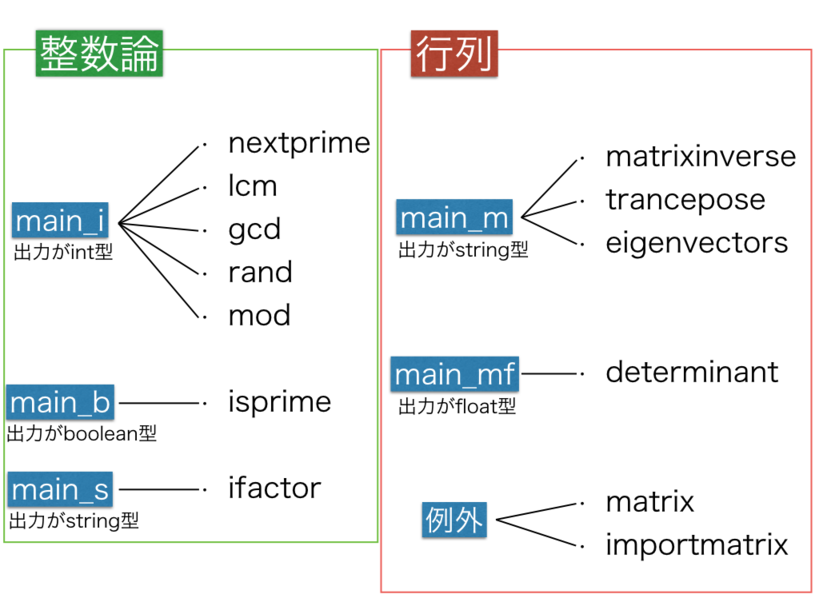
\includegraphics[width=12cm,bb= 0 0 937 753]{../figs/./mapleruby_eringi.007.png}
\caption{関数の分類.}
\label{figure:five}
\label{default}\end{center}\end{figure}
matrixは他にexec\_m(b)を使う関数がないため,importmatrixは他と重複するコードがないため例外としている.

